\documentclass[a4paper,11pt]{article}
\usepackage[T1]{fontenc}
\usepackage[utf8]{inputenc}
\usepackage{lmodern}
\usepackage{csquotes}

\usepackage{hyperref}
\usepackage{graphicx}
\usepackage[english]{babel}

\usepackage{graphicx}
\graphicspath{ {../Images/} }

% Defines how the section reference looks
\newcommand{\sectiondescribe}[1]{(Sektion {#1})}
\newcommand{\imagedescribe}[1]{(Bild {#1})}
\addto\captionsenglish{\renewcommand{\figurename}{Bild}}

\title{\Huge \textbf{Äventyr i Norgeria}}
\author{\textsc{Josef Utbult}}

\begin{document}
\pagenumbering{roman}
\maketitle
\newpage
\tableofcontents
\newpage
\pagenumbering{arabic}
%
\section{Bakgrund}
\subsection{Inledning}
\textit{Norgeria} är ett fiktivt land skapat av mig, Josef Utbult, för min D\&D 5e kampanj. Norgeria är ett försök till att koka ihop mina egna idéer samt en rad gamla och nya koncept som jag lånat från olika håll. 

\subsection{Början av ett äventyr}

\section*{Fångar på fri fot}

\begin{itemize}
	\item Ni är fångar som flytt från era vakter (alla utom en)
	\item Hur rymde ni?
	\item Ni sitter på Den glada abborren i hamnstaden Haggesund
	\item En av er är bara fett full och har råkat satt sig vid fel bord
	\item Alla förutom fyllot har förlorat hela sitt inventory, speciellt alla pengar
\end{itemize}

\subsection{Geografi}
Norgeria är en av de mer nordliga länderna i världen \textit{Vaerlden}. Ost om Norgeria ligger ett öde land kallat \textit{Svargeria}. Svargeria är ett kallt landskap fullt med vild uråldrig skog. De enda som bor i Svargeria är \textit{Svargarna}, olika små grupper och byar av nomadstammar. Söder om Norgeria ligger \textit{Dhee Ahrrg}, ett land lika vilt som Svargeria, men populerat av orcher. Ifrån Dhee Ahrrg seglar ibland rövartåg till kustbyarna i Norgeria för att plundra.

\section*{Gudar och Magi}
\subsection*{Gudar}
Gudar är ett osäkert ämne i Norgeria. Det verkar inte finnas några gudar på det materiella planet som intrigerar med invånarna i Norgeria. Därför finns det ingen definitiv sanning om gudar och religion, men detta är ingen anledning att inte vara oense i frågan. Olika individer och grupper tillber olika gudar och entiteter som de menar är de rätta. Vissa tror på en gud, vissa på ett antal och vissa är ateister som tror på naturkrafter och mindre entiteter. 

\subsection*{Magi}
Magi är ett fenomen som förekommer i Norgeria, om ens sällan. Magiker är ett sällsynt fenomen, men de finns i några olika former. Vissa har en naturlig känsla för magi och vissa har breda modeller och idéer om magins natur, men det finns ingen universell sanning kring magi. 

Det händer att clerics, paladins och warlocks tillber entiteter och ber dem om hjälp eller tjänster. Dessa besvaras om och om igen, men exakt vad det är som händer är ingen säkerhet.

\subsubsection*{Relationer mellan religioner}
Det händer att clerics, paladins och warlocks tillber olika gudar i religioner som talar emot varandra. Dessa får ofta deras vädjan besvarade, även om de går emot de andra ber om. Många religiösa accepterar sin ovetskap men vissa försöker förklara bort det som besvaras av motsägande religioner. De anklagar ofta magiker under andra trosuppfattningar för häxkonst, djävulsdyrkan eller simpla trick.

\subsection{Raser}
\subsection*{Alver}
Alver är sällsynta i Norgeria, men det finns fästen för dem där de lever i exkluderande samhällen. De har ofta svårt att erkänna det men de ser på andra raser med avsmak. Det finns två större fästen, Tramsø, den vita staden och Jord I Rana, underjordens hemlighet. 
%
\subsubsection*{Alvernas skriftspråk}
De moderna alverna har två skriftspråk; Alvtext och Uråldrig Alv-skrift. Alvtext är det som används i modern tid och detta kan alla alver, samt vissa lärda, läsa och skriva. Uråldrig Alv-skrift är däremot ett utdött språk. Detta kan finnas i ruiner och på fornlämningar. Det är ett utdött språk, men det har återupptäcktes och översatts av högt uppsatt lärda alver. Det kan tydas till viss del, men det är oerhört få alver som är lärda inom detta.
%
\subsubsection*{De fördömdas sigil}
Alver har under tusentals år haft en egen vållad förbannelse över dem som ärvs vidare i generationer. Denne kallas De fördömdas sigill, som är en magisk formel ditsatt av uråldriga förfäder av de moderna alverna. De fördömdas sigil beskrivs enligt legenderna som följande. \\ \\
%
\textit{``Den alv som mördar en annan alv, eller direkt bidrar till hans död, blir för evigt bränd med de fördömdas sigil.''} \\ \\ 
%
De märke som uppstår är en tatuering av ett runt sigill. Detta sigill innefattar skript som beskriver omständigheter runt alvens mord på i alvernas uråldriga skriftspråk.
%
Att ha de fördömdas sigil anses oerhört tabu, då mördandet av en alv ses som det värsta brottet som kan genomföras enligt alver. Alver med ett sigill blir disowned av alla andra alver och utstötta ur alvsammhället. 
%
Ett undantag till detta är alver som fått ett sigill i tjänst av sitt alvrike, då överhuvudet av riket tatuerat in sitt märke i form av sitt förlåtande runt sigillet för att deras synd, enligt dem, ska nollställas. Dessa blir inte disowned, men många alver ser fortfarande ner på alver med denna markering. 


\subsection*{Mört-män}
Baserad på rasen Kua-Toa från \textit{Monster Manual D\&D 5e\cite{MonsterManual}} \\
\url{https://www.dandwiki.com/wiki/Kuo-Toa_(5e_Race)}
%
\subsubsection*{Utseende}
Mört-män är något kortare än människor (medium). De har grå hud, stora gula ögon som skelar och händer samt fötter med simhud och svarta klor. Mört-män är kallblodiga och fuktiga. De uppskattar värme och hög luftfuktighet, varma bad, bastu och eldar.
%
\subsubsection*{Historia}
För hundratals år sedan levde Mört-männen i större samhällen och städer runt Norgerias kuster. Deras magiska och teknologiska egenskaper var på liknande nivå som den moderna människans samhälle, men det är sedan länge bortglömt. Nu lever de i mindre samhällen under ytan.
%
\subsubsection*{Egenskaper}
\textbf{Ability Score Increase.} Your Strength score increases by 2, and your Wisdom score increases by 1. \\
\textbf{Age.} The Kuo-toa age a bit faster than humans, reaching maturity at age 7 and living around half a century. \\
\textbf{Amphibious.} You can breathe in both air and water. \\
\textbf{Darkvision.} You are accustomed to the darkness of the Underdark, where daylight has no power. You can see in dim light within 120 feet of you as if it were bright light, and in darkness 
as if it were dim light. You can't discern color in darkness, only shades of gray. \\
\textbf{Slippery.} You have advantage on Dexterity (Acrobatics) checks and saving throws to escape a grapple or grapple attempt. \\

\begin{figure}
	\centering
	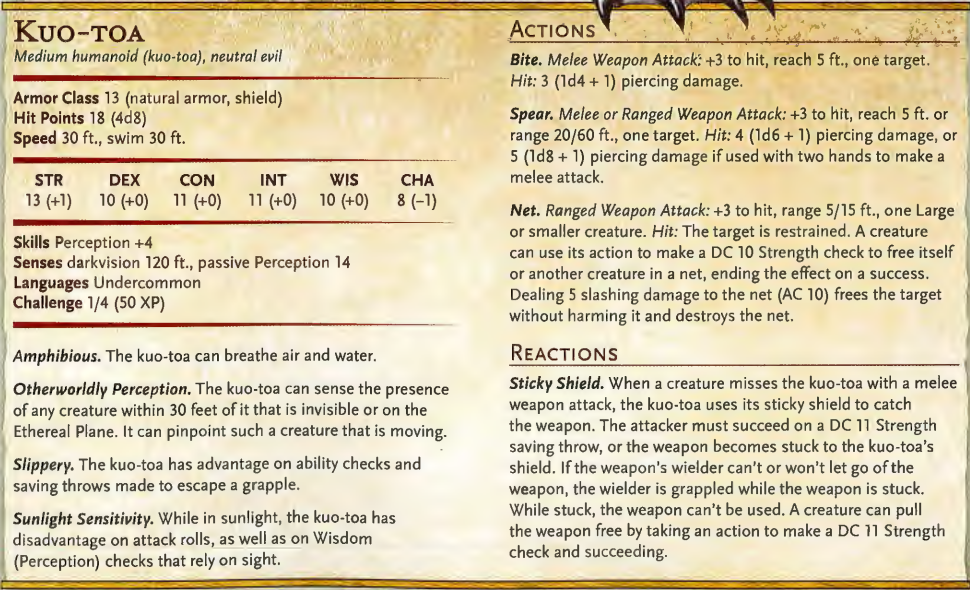
\includegraphics[width=\textwidth]{MortMan}
	\caption{\textit{Kuo-Toa} from \textit{Monster Manual D\&D 5e}\cite{MonsterManual}}
\end{figure}
\newpage
%
\section{Platser}
\subsection{Borgen}
\label{borgen}
Fängelset Borgen
\subsection{Bergen Bredvid Borgen}
\label{bergenBredvidBorgen}
Öst om \textit{Borgen} ligger \textit{Bergen Bredvid Borgen}. Dessa är några av de högsta bergen i södra Norgeria. Foten av berget upp ungefär halvägs är populerat av granskog, och resterande del av berget är tundra. Det sägs att dånande skrik av gigantiska örnar kan höras från ovan molnen runt bergstopparna.

\subsubsection{Bergsvakt Bengt}
Vid södra foten av det högsta berget bor Bergsvakten Bengt. Hanns stuga är en liten men trevlig sådan. Det finns plats för en säng, en kamin samt ett bord. Bengt vet bästa vägen upp för det högsta berget och vilka faror som lurar där. Han tror också på att det finns griffins uppe på det högsta berget. För 2 SP per dag så kan han agera guide upp på berget.

\subsubsection{Yetis}
Uppe på berget ovan trädgränsen lever yetis i massiva grottor. Yetis är rädda för eld och kommer inte nära lägereldar frivilligt. De har dock en tendens att smyga upp bakom människor som inte är på sin vakt och gå till attack.

\subsubsection{Griffins}
Högst upp på det högsta berget finns det en stor grotta. I denna finns ett massivt bo där två griffins ruvar tre ägg. Honan vaktar äggen ständigt, men kan luras ut ur grottan med höga ljud. Hanen flyger regelbundet iväg för att samla mat, men kan dyka upp när som helst.
\subsection{Hardals Fästning}
Hardals fästning ligger i dalen Hardel, fem kilometer norr om Trollkarlen Torkels hem \sectiondescribe{\ref{torkelsStuga}}, och innehavs av Haggan Agda, Hardals Häxa \sectiondescribe{\ref{hagganAgda}}. Fästningen vaktas av goblins som verkar vara anställda av Agda. De resande kan försöka smita sig in i borgen, vilket gör Agda misstänksam om de hittas. De kan ta sig in med våld och de kan knacka på och be om att få komma in. Agda släpper gärna in dem om de inte är allt för sketchy. Om de ber om det bjuder hon på mat i matsalen och sovplats över natten i gästrummen.

Slottet har en liten innergård, två våningar och ett torn. I tornet är Agdas arbetsrum. På första våningen finns en hall, ett kök med mathiss, två gästrum och arbetarnas levnadsutrymme (hängmattor och lite bord). På andra våningen finns Agdas sovrum och en kombinerad salong samt matsal. 

\paragraph{Hallen}
Hallen är ganska stor och öppen med en trappa längst med motsatt vägg från ingången. Den har två dörrar på vänster sida till vardera gästrum och en på högersidan till arbetarnas levnadsutrymme. I ett hörn står en byrå och i ett annat står en uppstoppad björn. Denna uppstoppade björn kan animeras av agda, vilket kräver en action av henne. Då spelar denne som en alierad björn till henne, men med alla fördelar av en odöd.

\paragraph{Gästrummen}
Gästrummen innehåller en stor säng, en eldstad och en byrå vardera. I ett av rummen finns en tavla med en gammal alv-kvinna på. 

\paragraph{Arbetarnas levnadsutrymme}
Arbetarnas levnadsutrymme är goblinarnas rum. Det sitter fyra goblins runt bordet och två ligger i varsin hängmatta. Det finns tio hängmattor hängda längst väggar och upphissade i taket och ett runt bord med stolar. Det finns även en kista med ett höftskynke i och något kopparmynt. Runt väggarna står två spjut, två svärd och tre armborst med varsit hölster.

\paragraph{Salongen}
I salongen finns ett stort bord med stolar och en soffgrupp runt en eldstad. Bokhyllor står längst med alla väggar som är fyllda med diverse böcker. Över eldstaden hänger ett magiskt svärd. 

\paragraph{Arbetsrummet}
Arbetsrummet har mängder av arbetsbänkar, avlastningsbord och hyllor. Dessa är fyllda mad papper, flaskor och småsaker. Om man letar på ytorna finns en skalle av guld (20 GP), samt 20 SP. Det finns även en bok med följande trollformler; Counterspell, Detect magic, Dispel Magic, Protection from Evil and Good, Remove Curse, See Invisibility. Det finns även en \textit{Låda med råttor} \sectiondescribe{\ref{ladaMedRattor}}
\subsection{Håggesund}
\label{haggesund}
%
Håggesund är en hamnstad på sydvästkusten i landet \textit{Norgeria}. Det är i stort sätt självförsörjande, men exporterar lite fisk samt fartyg och båtar från \textit{Bröderna Bågs Båtbyggeri} \sectiondescribe{\ref{brodernaBagsBatbryggeri}}. 
Alla byggnader i Haugesund är byggda i äldre förgrånat trä och är något slitna, likt en gammal nordlig fiskarstad.
%
\begin{figure}
	\centering
	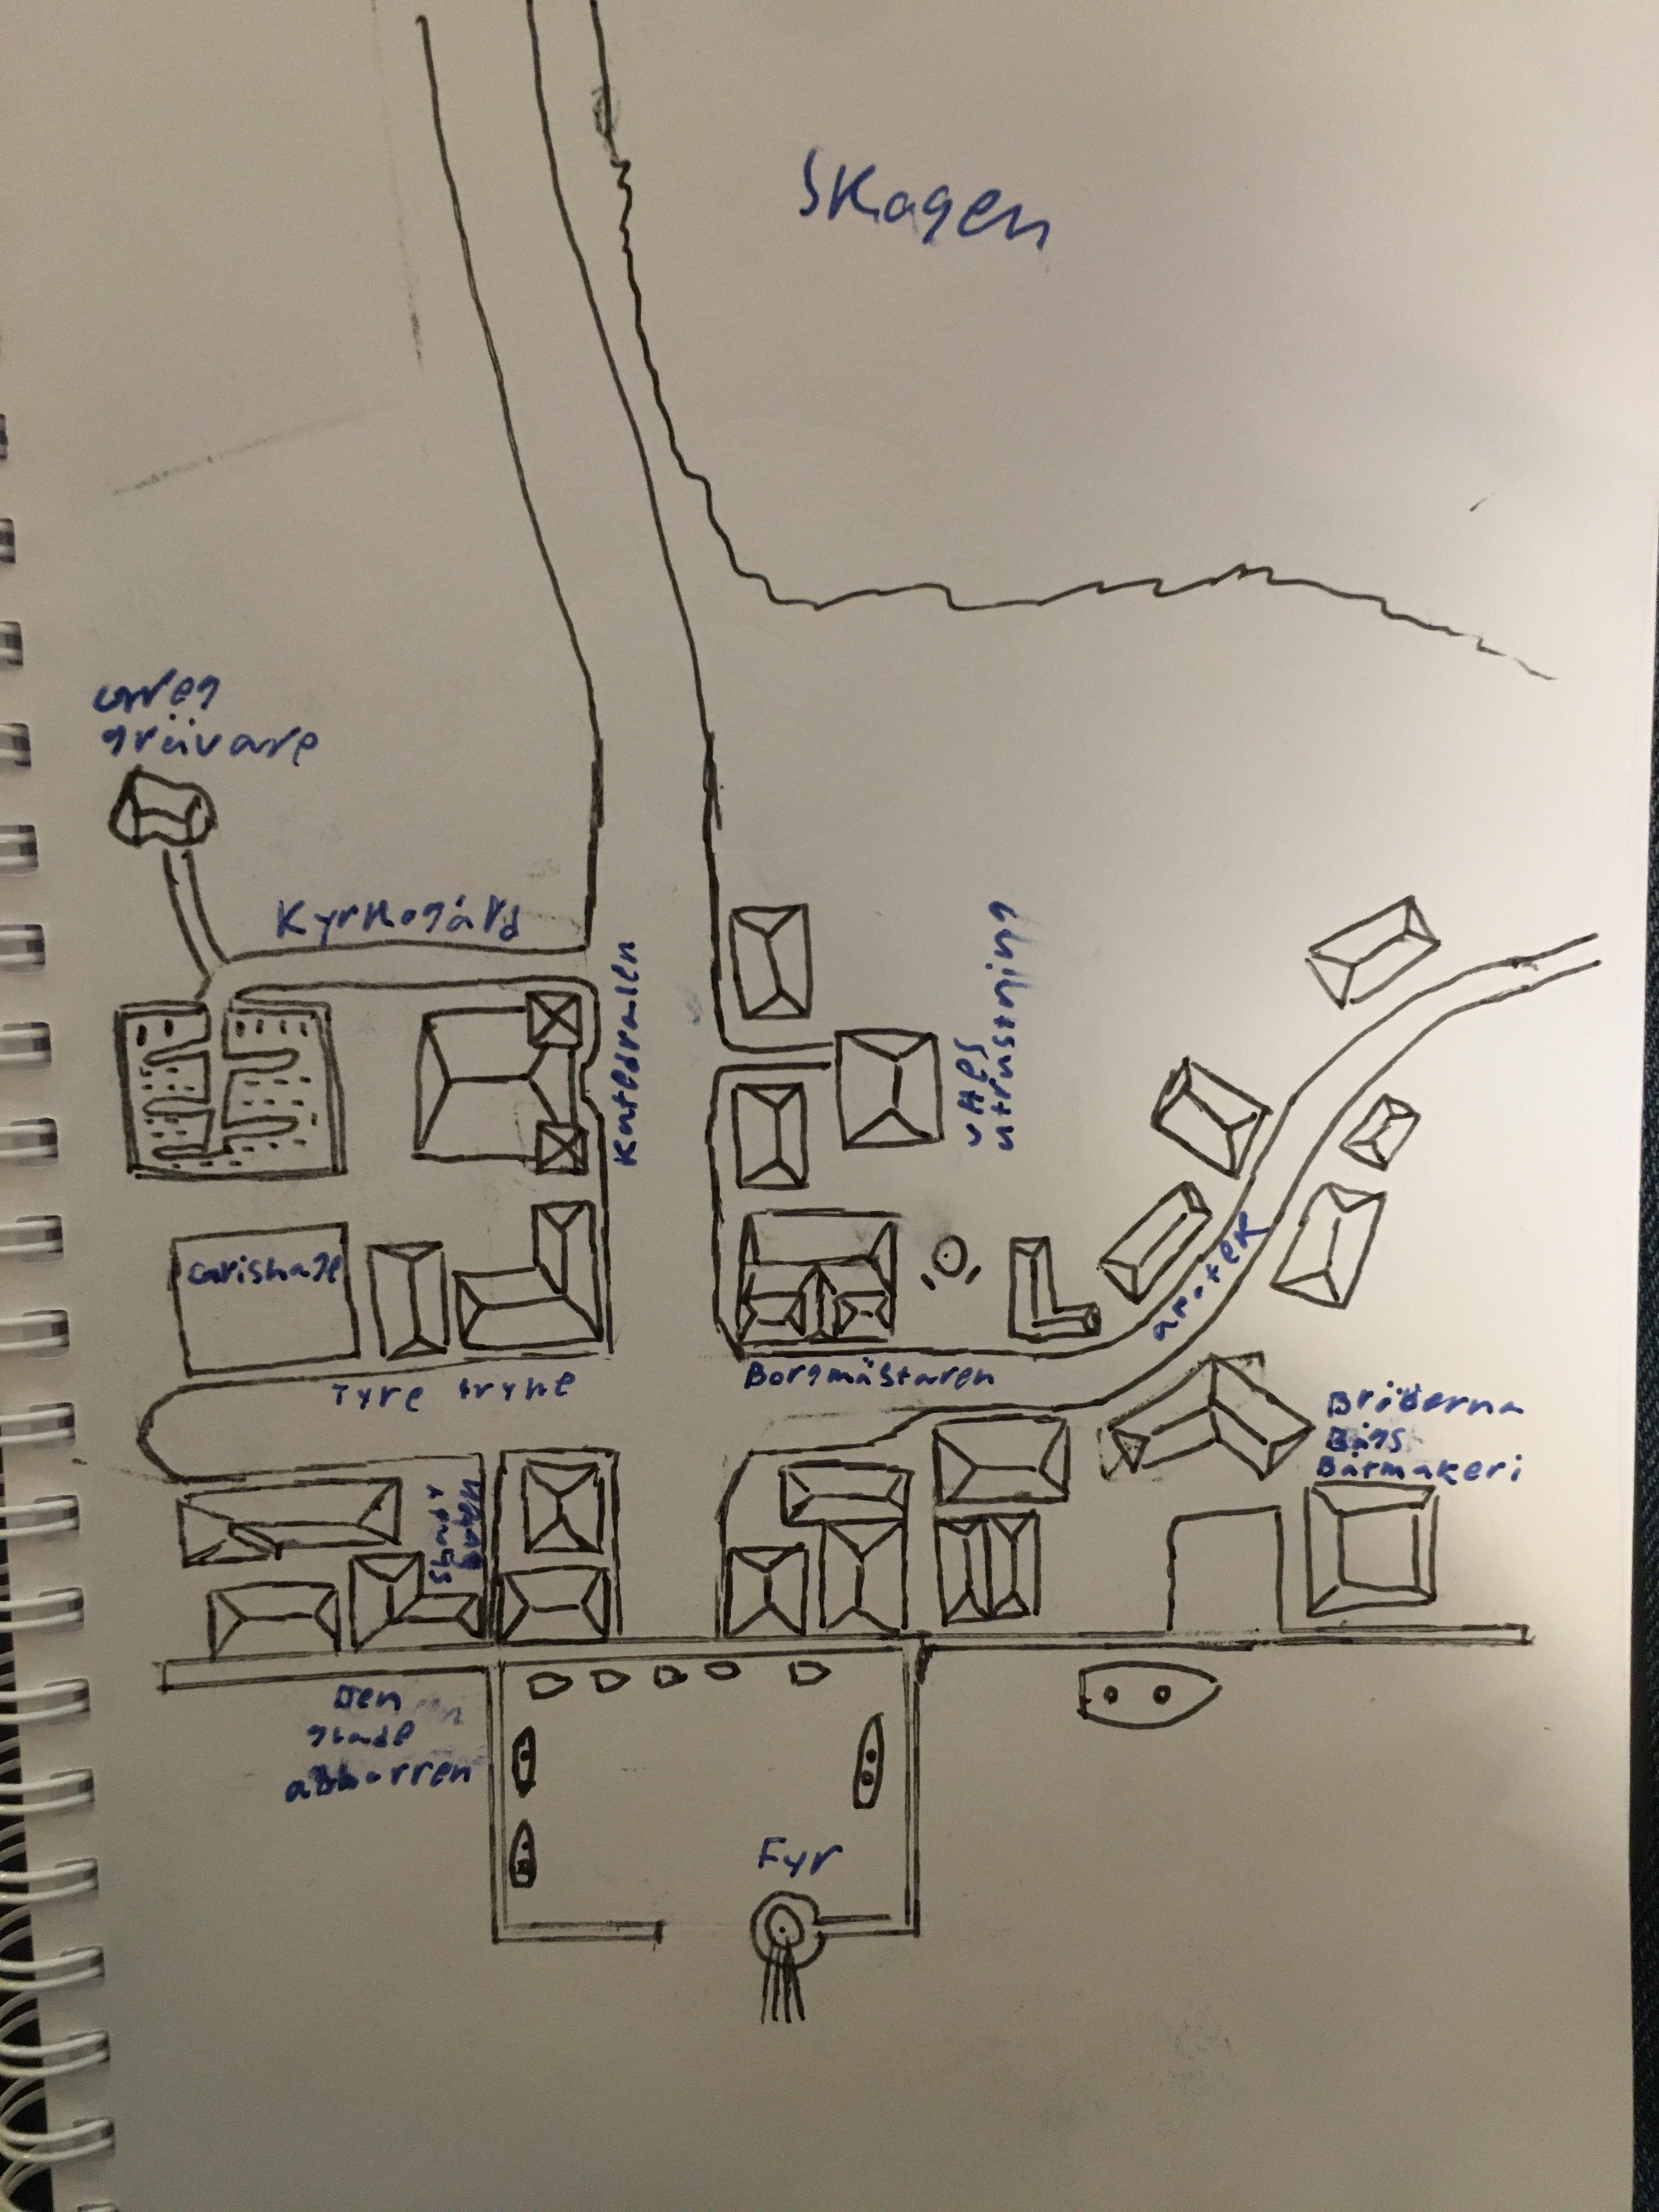
\includegraphics[width=\textwidth]{Haggesund}
	\caption{Håggesund}
\end{figure}
%
\subsubsection{Den glada abborren}
\label{haggesund:denGladaAbborren}
Den glada abborren är ett värdshus som ägs av Oskar, en högljudd kraftig man med flint och ölmage. Det finns utställt stolar och bord i det stora rummet och en bar längst in. I ett av hörnen finns en brinnande eldstad med en grupp fåtöljer. 
%
\paragraph{Mörtmannen Gurgler}
I en av fåtöljerna sitter en Mört-man \sectiondescribe{\ref{mortman}}, Gurgeler, med en huva för att dölja sin ras. Han är inte jättetaggad på att prata med äventyrarna, men kan berätta att han är en köpman från Mehec’ger, 
en by i havet utanför Haugesund. Han har tio guld på sig från handel % TODO: Vad säljer Gurgler?
%
\subsubsection{Borgmästarens hus/Stadshuset}
Borgmästare Korre Upt bor i stadshuset, en av de större byggnaderna i Håggesund. Stadshuset är lågt upplyst och utsmyckat med färglada tyger samt tavlor föreställande Griffins. I den stora salen i mitten av stadshuset sitter Korre Upt i en soffgrupp tillsammans med två andra överviktiga män. Dessa är Korres rådgivare som sitter och röker pipa i varsin soffa.

Korre är en kort liten man med oljigt svart hår samt en lång, tunn mustasch. Korre har en oerhörd fascination av Griffins, och har ett uppdrag angående dessa \sectiondescribe{\ref{korresGriffins}}.
%
\subsubsection{Apoteket}
Apotekare August säljer påfyllning till Medical Kits, Potion of healing och lite grundläggande magiska örter.
%
\subsubsection{Shady Sven}
Shady Sven säljer knark.
% TODO: Utveckla Shady Sven
%
\subsubsection{Tyre Tryne och hans grishage}
% TODO: Skriv om Tyre Trynes grishage. 
Mocka bajs för silvermynt.
%
\subsubsection{Bröderna Bågs Båtmakeri}
\label{brodernaBagsBatbryggeri}
% TODO: Skriv om Bröderna Bågs Båtmakeri
%
\subsubsection{Uffes utrustning}
% TODO: Skriv om uffes utrustning
%
\subsubsection{Katedralen}
Präst
Tillber Den Djupe
Den djupe sägs leva i ett sjunket skepp någonstans i havet långt utanför Haugesund
Där samlar han på skatter som sjunkit till havsbotten
% TODO: Utveckla Katedralen, presten och religionen i Håggesund
%
\subsubsection{Kyrkogård}
% TODO: Skriv nått om kyrkogården
% 
\subsubsection{Greg Gravgrävare}
% TODO: Skriv om Greg Grävare till mer flytande stilP
Gregs hus är liten och väldigt sliten. Där inne är det fullt med bråte och luktar unket. Det finns tre fönster utan gardiner. På fönsterkarmarna står det glasburkar med namn skrivna på och gulvit vätska i som har sjunkit till botten. Det är Gregs säd.

Greg är nekrofil. Han mastruberar till döda kvinnor och sorterar samt lagrar sin säd i burkar med deras namn på. Detta berättar han gärna om och blir exalterad om man frågar om det. Greg skäms inte.


\subsection{Mehec’ger}
% TODO: Lägg till stad
\subsection{Ostlo}
\subsubsection{Beholderkult}
I Ostlo smyger en grupp kultmedlemmar runt i skuggorna. De tillber \textit{Ögat}, en stor beholder som lever i katakomberna under staden. Kultmedlemmarna klär sig i röda dräkter med huvor, har rakade huvuden och ett öga tatuerat i pannan. Dessa spelas som en \textit{Cult Fanatic} \imagedescribe{\ref{img:cultFanatic}} ifrån Monster Manual \cite{MonsterManual}. De rör sig i gränder och mer laglösa värdshusen i Ostlo. De gillar att stjäla magiska föremål, specielt spelares arcane focus, och kan försöka stjäla dessa från spelarna.
%
\subsubsection{Ögat}
\begin{displayquote}
En mörkt marinblå klump svävar några decimeter över marken. Den har ett gigantiskt gult öga, en enorm mun med taggiga tänder och tentakler utstretande från sig med små ögon i ändarna.
\end{displayquote}
\textit{Ögat} är en beholder \imagedescribe{\ref{img:beholder}} som lever i katakomberna under Ostlo. Denna är ledaren för beholderkulten och samlar magiska artefakter i en hög bakom sig. Beholdern konverserar gärna med äventyrarna innan den anfaller dem, han är väldigt egosentrisk och har storhetsvansinne, och pratar främst om sig själv.

\begin{figure}
	\centering
	\label{img:cultFanatic}
	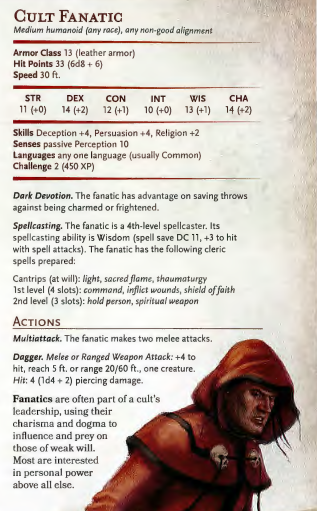
\includegraphics[width=\textwidth]{CultFanatic}
	\caption{\textit{Cult Fanatic} från \textit{Monster Manual D\&D 5e}\cite{MonsterManual}}
\end{figure}

\begin{figure}
	\centering
	\label{img:beholder}
	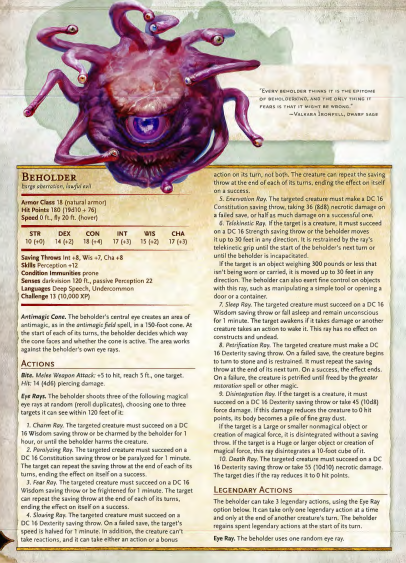
\includegraphics[width=\textwidth]{Beholder}
	\caption{\textit{Beholder} från \textit{Monster Manual D\&D 5e}\cite{MonsterManual}}
\end{figure}

\subsubsection{Katakomber under Ostlo}
Under Ostlo finns ett uråldrigt katatakombsystem. Detta var ursprungligen en kloak som användes av staden, men efter att detta fallit ur bruk har det tagits över av en Beholder som etablerat ett kultföljande. Följande rum finns i katakomberna.
%
\begin{enumerate}
	\item I en av de bredare kloakerna under Ostlo finns en ficka. Där finns en gammal port som är låst med ett stort gammalt lås. Bredvid sitter på var sida en slocknad fackla. Porten går att dyrka ganska lätt.
	\item 
	\item Här är en sovsal med tio våningssängar. Där finns även ett runt bord med stolar samt en eldstad. Det sitter tre kultister runt bordet samt tre i olika sängar. Alla utom två är beväpnade, men det finns vapen i rummet de kan hämta. Om man undersöker eldstaden kan man hitta en dold knapp, som öppnar en gång igenom eldstaden till en stege mot rum 10. För att gå igenom bör man släcka elden först. 
	\item Det här är den hemliga källaren under handelsboden Svarta Koftan. Det finns lagrat en del torkad mat, rep, facklor samt tre pilar i ett gammalt hölster.
	\item Det finns en stege ner till rum 9.
	\item En tänd fackla sitter mittemot gången mot rum 5. Om någon undersöker denna märker man att den går på ett gångjärn. Dras det i denna öppnas en hemlig dörr till rum 6. Där är det mörk, och det finns inga facklor där inne. Här finns en kista med 10 guld, 15 guld, 2 juveler. Det finns även en ringbrynja, en hjälm samt ett långsvärd.
	\item
	\item Igenom det här rummet rinner en flod kloakvatten, ner genom ett galler till rum 12. Gallret går att dra av och man kan ta sig igenom för varelser upp till liten storlek.
	\item 
	\item Här är en vinkällare. Det finns en kvast, 10 flaskor vin, 3 flaskor brännvin, 1 tunna mjöd, 10 limpor bröd samt 4 ostar. Går man upp mot rum 3 kan man skjuta upp den hemliga dörren, men det är svårt att ta sig ut om man inte lyckas få bort elden.
	\item 
	\item Här kommer det vatten från rum 8 till en liten pool med smutsigt vatten. I botten av polen ligger 3 kopparmynt. Polen flyter ut i en större kloak mot hamnen.
	\item Det här verkar vara någon form av skattkammare. Här finns en full tung rustning på en visningsdocka. Denna är i människostorlek, men kan modifieras enkelt till dvärgstorlek. Det finns 2 armborst, 20 armborst-boltar, två kortsvärd, en sköld, samt två kistor. En lista innehåller 3 sätt fina kläder och 3 munkdräkter. I den andra finns 15 guldmynt, 2 juveler och en liten ebonyststyett. 
	\item Det här är en stor sal med en upphöjd scen. På scenen flyter en stor Beholder. Denna är ledaren för kulten och samlar magiska artefakter i en hög bakom sig. Beholdern kallar sig ”Jag är” och konverserar gärna med äventyrarna innan den anfaller. Det finns även 3 kultister i salen som sjunger en hymn till Beholdern. Dessa anfaller med Beholdern.
\end{enumerate}

\subsection{Thear - Den dränkta staden}
\label{thear}
\subsection{Torkels stuga}
\label{torkelsStuga}
Torkels hus ligger två dagar norr om Håggesund. Hans hus är ett ganska stort trähus, men ganska slitet. Där inne är det fullt med olika saker och målningar på väggarna på olika alkemiska cirklar.
I mitten av rummet står ett fat med vatten och en lapp där det står något.
%
\begin{displayquote}
Är jag inte här så är det nog något som gått fel. Kan du vara så snäll att doppa en tå i fatet? Fördelaktigen en Alv-tå. Tack på förhand.
\end{displayquote}
%
Om någon doppar en tå materialiseras en trollkarl i ett rökmoln som säger poff. Den Tokiga Trollkarlen Torkel materialiseras. Trollkarlen blir av samma ras som tån som doppats, och blir ganska lik individen i fråga, men av manligt kön och gammal. Man blir uppskattad av Torkel om han blivit alv, men helt ok med att blivit människa. Han blir dock ganska grinig om han blivit gnom, halvman eller dvärg. Är han grinig är han inte jättetaggad på att prata, men han kan bli övertalad om man är lite karismatisk eller bjuder på mat eller vin. Torkel har ett uppdrag som äventyrarna kan välja att ta \sectiondescribe{magikerMedRelationsproblem}.
\subsection{Tramsø - Den vita staden}
%
Tramsø är en av de två, och den enda allmänt kända alvstaden i Norgeria. Tramsø bebos näst intill endast av överalver, med ytterst få lärda samt köpmän av andra raser. Tramsø består av en 200 meter hög mur, vit som snö, med själva staden på toppen. Exakt vad för teknik och magi som användes är för länge sedan bortglömt, men man vet att det för hundratusentals år sedan byggdes en mur runt ett berg, berget plattades till och muren fylldes upp för att skapa en cylindrisk platå på vilken staden byggdes. Staden är nästintill ointagbar då de enda vägarna upp är smala branta gångar längst med muren som är tungt försvarade.

Invånarna i Tramsø menar att staden styrs som en teknokrati, vilket det en gång varit, men efter hundratals år har de statliga organen stagnerat till att styras av en grupp ledarmöten som sitter på sin post livet ut: \textit{Rådet}. Dessa väljs in av resterande medlemmar och brukar allt som oftast vara arvtagare av de före detta ledamöterna. Rådet styr från \textit{Universitetet}, som ligger som centrum för staden.

\newpage
%
\section{Uppdrag}
\subsection{Magiker med relationsproblem}
\label{magikerMedRelationsproblem}
%
\subsubsection{Torkel den Tokiga Trollkarlen}
Torkel den Tokiga Trollkarlen är en gammal man av ursprungligen alv-ras. Han bor i en liten stuga norr om Håggesund \sectiondescribe{\ref{torkelsStuga}}.
%
\subsubsection{Torkels uppdrag}
Torkel har ett uppdrag till de resande. Hans ärkerival \textit{Haggan Agda, Hardals Häxa} har stulit hans slott, \textit{Hardals Fästning}, och tvingat honom bo i hans gamla håla, som han tidigare använt som förråd. Nu sitter han här och är grinig mestadels av tiden. Det äventyrarna kan göra för Torkel är att ta med en liten lila behållare med någon tjock vätska i till Hardals fästning och lura i Agda denna vätska. Den måste konsumeras och Agda får inte komma till onödig skada. Som belöning kan Torkel betala äventyrarna med 40 guldmynt, som han har i slottet. Frågar de något om Agda verkar han lite sur på henne men påpekar att hon är välldigt gästvänlig och gärna bjuder in resande på en måltid och plats över natten.
%
\subsubsection{Haggan Agda, Hardals Häxa}
\label{hagganAgda}
Agda är en kort, gammal människokvinna klädd i en rob som släpar efter henne. Hon är också en magiker som spenderar mestadels av sin tid i sitt arbetsrum och sin salong. Hon talar gärna med främlingar. Om någon frågar om hennes relation med Torkel nämner hon att den inte är så bra för tillfället. Hon säger att de föll isär för några år sedan vilket ledde till deras skilsmässa. Hon vill inte höra av Torkel mer efter det.

Om Äventyrarna får i Agda vätskan ser ni hur hon börjar darra. Stora bölder växer ut ur hela hennes kropp som växer till lämmar och ett huvud. Det slutar med att Agda förvandlats till Torkel, som snabbt trollar fram lite kläder till sig själv. Han tackar äventyrarna och hämtar deras guld åt dem. Goblinserna är något fientliga mot Torkel då Agda salt åt dem att hålla honom borta, men han påpekar att det är han som nu har allt guld och kan betala dem vilket mildrar dem. Vill de sova över natten så går det bra för Torkel då de hjälpt honom, men sedan vill han att de ska ut. 

\subsubsection{Agdas uppdrag}
Hela uppdraget kan göras igen, men nu med Agda som uppdragsgivare. Hon bor i Torkels stuga nu och ger dem en påse med torkade örter och en glasflaska med olja i. Örterna ska konsumeras av Torkel och efter det ska han smörjas i oljan. Vid konsumtion blir Torkel en groda, och när grodan smörjs blir denna Agda (med kläder). Torkel är dock inte villig att släppa in äventyrarna självmant då han ser igenom deras trick.

\subsection{Korres Griffins}
\label{korresGriffins}
Borgmästare Korre Upt är besatt av Griffins, och önskar inget annat än att äga en. Det sägs att det lever Griffins uppe på det högsta berget i \textit{Bergen Bredvid Borgen} \sectiondescribe{\ref{bergenBredvidBorgen}}. Korres uppdrag för spelarna är att ta sig upp på berget och ta med sig griffinägg till honnom. Korre betalar 100 GP per ägg som spelarna lyckas få med sig till honom.
\subsection{Över Tramsøs väggar}
\label{OverTramsosVaggar}
\textit{J'le Vare Fullmåne} söker äventyrare för att hjälpa honom med ett uppdrag; han och hans dotter, \textit{Ahna Le'blek Fullmåne}, behöver ta sig in till Tramsø. J'le Vare är nämmligen en politisk aktivist som varit aktiv länge i Tramsø, och förespråkade ideer som inte stämmde överrens med Rådets. Detta ledde till att J'le Vare blev dömd för ett brott han inte ansett sig begått och utkastad från staden. J'le Vare drömmer om att ta sig tillbaks in i Tramsø för att kunna bidra till motståndsrörelsen.

Men Tramsø är inte lätt att ta sig in i. Det finns endast en väg upp för berget som staden ligger på, denna vaktad och blockerad i flera steg. J'le Vare menar att smuggla sig in via vägen är omöjligt, och detta ger endast ett alternativ kvar. J'le Vare vill klättra upp för bergsväggen och undvika vägen så långt det går. Han, hans dotter och hans nära vän, \textit{Lias Krev} \sectiondescribe{\ref{liasKrev}}, ska med honom och de söker eskort. Lias har de utrustning som krävs för att klättra, och det han vill att ni ska göra är att oskadligöra vakter i det fallet att de skulle upptäckas.
%
\section{Föremål}
\subsection{Låda med råttor}
\label{ladaMedRattor}
Lådan med råttor är ett skrin av grovt trä med lock. I denna så materialiseras 1d6 råttor på en oregelbunden basis som försöker klättra ut ur den. Om det inte materialiserats råttor i den, eller om man bara kollar i den, ligger endast lite halm samt råttbajs.
%
\newpage

\begin{thebibliography}{9}

\bibitem{MonsterManual} 
Wizards of the Coast. 
\textit{Monster Manual: A Dungeons \& Dragons Core Rulebook}, 2014.

\end{thebibliography}


% \begin{chapquote}{Author's name, \textit{Source of this quote}}
% ``This is a quote and I don't know who said this.''
% \end{chapquote}

\end{document}
